\documentclass[a4paper,12pt]{report}
\usepackage{myStyle}
%\usepackage[utf8]{inputenc}
%\usepackage{a4wide}
%\usepackage[pagebackref,colorlinks=true,urlcolor=blue,linkcolor=blue,citecolor=blue]{hyperref}
%\usepackage{mathptmx}
%\usepackage{amsmath}
%\usepackage{amssymb}
%\usepackage{amsfonts}
%\usepackage{amscd}
%\usepackage{amsthm}
%\usepackage{amsxtra}
%\usepackage{mathrsfs}
%\usepackage{bbold}
%\usepackage{nicefrac}
%\usepackage{graphicx}
%\usepackage{xcolor}
%\usepackage[shortlabels]{enumitem}
%\usepackage{mathtools}
%
%\usepackage[bf]{titlesec}
%% \renewcommand{\thesection}{\Roman{section}}
%\titleformat{\section}{\large\bfseries}{\thesection.}{1em}{}
%\titleformat{\subsection}{\bfseries}{\thesubsection.}{1em}{}
%\titleformat{\subsubsection}{\sl}{\thesubsubsection.}{1em}{}
%% \titleformat{\paragraph}{}{\theparagraph}{}{}
%% \titleformat{\appendix}{}{}{}{blah}
%% \titleformat{\subparagraph}{}{}{0pt}{}
%
%
%\usepackage[norelsize,boxed,noend,linesnumbered]{algorithm2e}
%\DontPrintSemicolon
%\SetKwFor{RepeatTimes}{repeat}{times}{endrepeat}
%%\RestyleAlgo{ruled}
%% 'norelsize' takes care of incompatibility with amsart in old version of algorithm2e.
%%             Remove it once the new version is on the system
%% \begin{algorithm}[htbp OR H]
%% Commands: \TitleOfAlgo{} \For{}{} \Foreach{}{} \If{}{} \eIf{}{}{} \EsleIf{}{} \While{}{} \Return{}
%\newcommand{\eqdef}{\stackrel{\rm def}{=}}
%
%\theoremstyle{plain}
%\newtheorem{theorem}{Theorem}
%\newtheorem*{theorem*}{Theorem}
%\newtheorem{proposition}[theorem]{Proposition}
%\newtheorem*{proposition*}{Proposition}
%\newtheorem{corollary}[theorem]{Corollary}
%\newtheorem*{corollary*}{Corollary}
%\newtheorem{lemma}[theorem]{Lemma}
%\newtheorem*{lemma*}{Lemma}
%\theoremstyle{definition}
%\newtheorem{definition}[theorem]{Definition}
%\newtheorem*{definition*}{Definition}
%\newtheorem{example}[theorem]{Example}
%\newtheorem*{example*}{Example}
%\theoremstyle{remark}
%\newtheorem{remark}[theorem]{Remark}
%\newtheorem*{remark*}{Remark}
%
%\numberwithin{theorem}{section}
%
%
%\newcommand{\CC}{\mathbb{C}}
%\newcommand{\NN}{\mathbb{N}}
%\newcommand{\QQ}{\mathbb{Q}}
%\newcommand{\RR}{\mathbb{R}}
%\newcommand{\ZZ}{\mathbb{Z}}
%\newcommand{\kk}{\mathbb{k}}
%\newcommand{\FF}{\mathbb{F}}
%\newcommand{\EE}{\mathbb{E}}
%
%%% E x p e c t a t i o n
%\DeclareMathOperator*{\Prb}{\mathbf{P}}
%\DeclareMathOperator*{\Exp}{\mathbf{E}}
%\DeclareMathOperator*{\HExp}{\text{\huge$\mathbf{E}$}}
%\DeclareMathOperator*{\LExp}{\text{\Large$\mathbf{E}$}}
%\DeclareMathOperator*{\Var}{\mathbf{D}}
%\DeclareMathOperator*{\Covar}{\mathbf{Covar}}
%\DeclareMathOperator{\IndicatorOp}{\mathbf{I}}
%\newcommand{\Ind}{\IndicatorOp}
%\newcommand{\Cov}{\Covar}
%
%\DeclarePairedDelimiter\bra{\langle}{\rvert}
%\DeclarePairedDelimiter\ket{\lvert}{\rangle}
%\DeclarePairedDelimiterX\braket[2]{\langle}{\rangle}{#1 \delimsize\vert #2}
%
%\newcommand{\comment}[1]{\text{\footnotesize[#1]}}

\usepackage{lscape}
\begin{document}
\title{MTMS.01.088 Mitmemõõtmeline analüüs\\Faktoranalüüs\\Projekt}% <<== CHANGE THIS
\author{Anti Ingel}% <<== CHANGE THIS

\date{\today}
\maketitle

\chapter{Sissejuhatus}

%\subsection{Aju-arvuti liides}

Töö eesmärgiks on proovida faktoranalüüsi kasutades täiendada autori varasemat tööd, milleks on visuaalselt esilekutsutud potentsiaalidel (VEP) põhinev aju-arvuti liides (AAL). AALiks nimetatakse aju ning arvuti vahelist otsest suhtluskanalit ehk tavaliselt arvutiprogrammi, mis saab sisendi kasutaja ajust. Seega kasutaja ei pea arvutiga suhtlemiseks vajutama nuppudele, vaid ajus esile kutsuma teatud signaali, mida on võimalik aju tegevuse salvestamiseks mõeldud seadmetega mõõta ning salvestusest tuvastada.

Kasutaja ajutegevuse mõõtmiseks kasutatakse tavaliselt elektroentsefalograafiat (EEG), kuna võrreldes teiste meetoditega on EEG muutunud väga odavaks ning viimasel ajal on lisaks professionaalsetele seadmetele välja tulnud ka tarbijatele orienteeritud kasutajasõbralikke seadmeid.

Et EEG salvestuse põhjal otsustada, millist käsku kasutaja arvutile edastada soovib, tuleb salvestusest eraldada tunnused. VEPil põhinevad AALid jagunevad omakorda erinevat tüüpi AALideks vastavalt sellele, kuidas VEP ajus esile kutsutakse ning seejärel EEG salvestusest tuvastatakse. Üks populaarsemaid viise on kasutada sagedusel põhinevaid VEPe, mille puhul on EEG signaalist eraldatavateks tunnusteks kindlad sagedused. Igale käsule, mida kasutaja saab arvutile edastada vastab kindel sagedus. Sagedus kutsutakse ajus esile visuaalse stiimuliga, mida näidatakse kasutajale arvuti ekraanil.

Antud AAL põhinebki sagedustel ning kasutab elektroentsefalogrammist tunnuste eraldamiseks kahte erinevat meetodit---võimsusspektri analüüsi ning kanoonilist korrelatsioonanalüüsi. Kanoonilise korrelatsioonanalüüsi meetod arvutab igale käsu sagedusele vastava kanoonilise korrelatsiooni EEG signaaliga. Võimsusspektri analüüsi meetodiga saab aga kindlaks teha kui palju käsule vastavat sagedust EEG signaalis on.
%Kuna EEG on mitmekanaliline, siis võimsusspektri analüüsi meetod annab iga käsu kohta nii mitu tulemust, kui mitu EEG kanalit signaali mõõtmiseks kasutati.

Lõpuks tuleb saadud tunnuste põhjal otsustada, millist käsku soovis kasutaja arvutile edastada. Ilmselt mida suurem on kanooniline korrelatsioon vastava käsu sagedusel EEG signaaliga ning mida rohkem vastava käsu sagedust EEG signaalis on, seda suurema tõenäosusega soovis kasutaja just seda käsku edastada. Aga kuna meetodeid on mitu ja kumbki meetod eraldab tunnuseid iga käsu kohta, siis tulemuseks on hulk tunnuseid, mida on raske interpreteerida.

Kuna varasemalt taolist erinevate tunnuste eraldamise kombineerimist tehtud ei ole, siis olemasolevast kirjandusest on vähe abi ning siit tekibki küsimus---kuidas kõigi nende saadud tunnuste põhjal teha lõplik otsus, millist käsku kasutaja soovis edastada? Kas mõlemal meetodil peaks olema võrdne kaal lõpliku otsuse tegemisel või ühel neist suurem? Kui palju peaks suurim korrelatsioon/võimsus olema teistest parem?

Taoliste küsimuste jaoks vastuse saamiseks proovingi kasutada faktoranalüüsi, et esitada eraldatud tunnused vähemate tunnuste kaudu ning seeläbi lihtsustada kasutaja edastatud käsu kindlaks tegemist.

\chapter{Andmete kirjeldus}

Kuna töö eesmärgiks on autori enda kirjutatud AALi täiendamine, siis ka andmed on autori enda kogutud. Andmed ise ning spetsiifilisemad detailid on lisas~\ref{lisa1}.

\section{Elektroentsefalogramm}

EEG signaali mõõtmiseks kasutati Emotiv EPOC seadet, mille mõõtmissagedus on 128 Hz ning 14 võimalikust sensorist kasutati ainult nelja sensorit, mille asukohad on 10-20 elektroodide paigutamise süsteemi järgi P7, O1, O2 ja P8. Need sensorid valiti, kuna asuvad nägemiskeskusele kõige lähemal ja seega on parimad VEPide tuvastamiseks. Täielikud EEG seadme spetsifikatsioonid on Emotivi kodulehel\footnote{https://emotiv.com/product-specs/Emotiv\%20EPOC\%20Specifications\%202014.pdf}.

EEG signaal AALi kasutamise ajal salvestati viielt tervelt inimeselt, kellel varasem AALi kasutamise kogemus puudus. Edasises analüüsis kasutatakse ainult ühe inimese EEG signaali, kuna erinevate inimeste EEG signaal erineb. Üks signaal valiti välja selle põhjal, millel kõige selgemalt alfa-lained ülejäänud signaalist eristusid.

EEG signaali andmestikus on tunnusteks EEG sensorite asukohad 10-20 elektroodide paigutamise süsteemi järgi ning vaatlusteks on vastava sensori mõõdetud pinge erinevus tugisensori mõõdetud pingest mikrovoltides iga $\frac{1}{128}$ sekundi järel, mille sisse on arvestatud ka $4000 \mu$V nihe.

\section{Visuaalselt esilekutsutud potentsiaalid}

VEPide esilekutsumiseks, st kasutajale visuaalsete stiimulite näitamiseks kasutati 14-tollist 60 Hz sagedusega 1600x900 resolutsiooniga monitori. Täielikud monitori spetsifikatsioonid on HP kodulehel\footnote{http://h71016.www7.hp.com/dstore/html/pdfs/AMS\_HP\_EliteBook\_840\_G1\_Notebook\_PC\_Data\_Sheet.pdf}.

EEG salvestamise ajal sai kasutaja edastada arvutile kolme erinevat käsku, nendele vastavad sagedused olid 6.67 Hz, 7.5 Hz ning 8.57 Hz. Käskude edastamise järjestus, mida kasutaja pidi järgima, oli arvuti poolt juhuslikult genereeritud ning kasutajale eksperimendi jooksul käsk-käsu haaval ekraanil näidatud. Seega kasutaja proovis edastada käske kindlas järjestuses ning edastatav käsk vahetus kindla aja möödudes. Seega on teada mis aja hetkel millist käsku kasutaja arvutile edastada proovis.

\section{Eraldatud tunnused}

EEG signaalist on omakorda eraldatud tunnused. Kanoonilise korrelatsioonimeetodiga on iga käsu jaoks iga $\frac{1}{128}$ sekundi järel arvutatud käsu sageduse ja EEG signaali vaheline kanooniline korrelatsioon. Võimsusspektri analüüsi meetodiga on iga käsu jaoks iga $\frac{1}{128}$ sekundi järel arvutatud käsule vastava sageduse hulk EEG signaalis tugisensori signaali suhtes, ühikuks on $\left(\frac{\mu V ^2}{Hz}\right)$. Lisaks käsu enda sagedusele, arvutab võimsusspektri analüüsi meetod ka tunnuse iga käsu sageduse teise harmooniku jaoks, kuna teise harmooniku hulk signaalis see aitab kasutaja käsku kindlaks teha.

Andmestikus kasutatavad lühendid
\begin{itemize}
	\item CCA - kanooniline korrelatsioonanalüüs
	\item PSDA - võimsusspektri analüüs
	\item f1 - sagedus 1
	\item h1 - sageduse esimene harmoonik (ainult võimsusspektri analüüsi puhul)
	\item sum - tulemus summeeritud üle harmoonikute (ainult võimsusspektri analüüsi puhul).
\end{itemize}
Näiteks tunnuse CCA\_f1 väärtus 0.8 tähendab, et vaadeldaval ajahetkel oli EEG signaali ja 1. käsu sagedusega (6.67 Hz) sinusoidi kanooniline korrelatsioon 0.8. Käsu kindlaks tegemiseks võib näiteks võrrelda tunnuste CCA\_f1, CCA\_f2 ja CCA\_f3 väärtuseid ja valida nende hulgast suurima väärtusega tunnus.

Näiteks tunnuse PSDA\_h2\_f3 väärtus näitab aga kui palju 3. käsu sageduse (8.57 Hz) teist harmoonikut ($8.57\cdot2=17.14$ Hz) vaadeldaval ajahetkel signaalis on. Jällegi võib võrrelda kõiki antud meetodi tunnuste väärtuseid iga käsu kohta, st tunnuste PSDA\_h2\_f1, PSDA\_h2\_f2, PSDA\_h2\_f3 väärtuseid ning valida nende hulgast suurim, et kindlaks teha, millist käsku kasutaja selle meetodi arvates edastada tahtis.

Tahame aga mõlemad meetodid koos tööle panna ja üks võimalus seda teha on omistada igale tunnusele oma kaal, kui palju antud tunnus lõplikku otsust mõjutab. Selleks proovimegi kasutada faktoranalüüsi.

%EEG salvestati kolme eraldi katsena, katsede vahel olid paariminutilised pausid.
%\begin{table}[h!]
%	\begin{tabular}{|l|l|l|l|}\hline
%		Katse & Tunnuseid & Vaatluseid & Kestvus (s) \\\hline
%		1	  &	4		  & 12656	   & 98 \\\hline
%		2	  & 4		  & 10688	   & 83 \\\hline
%		3	  & 4		  & 12140	   & 94 \\\hline
%	\end{tabular}
%\end{table}

%EEG signaalist on omakorda eraldatud tunnused---iga käsu sagedusele vastav kanooniline korrelatsioon ja igale käsule vastava sageduse hulk $\left(\frac{\mu V ^2}{Hz}\right)$ signaalis tugisensori signaali suhtes esimese kahe harmooniku kohta.

\begin{figure}[h!]
	\centering
	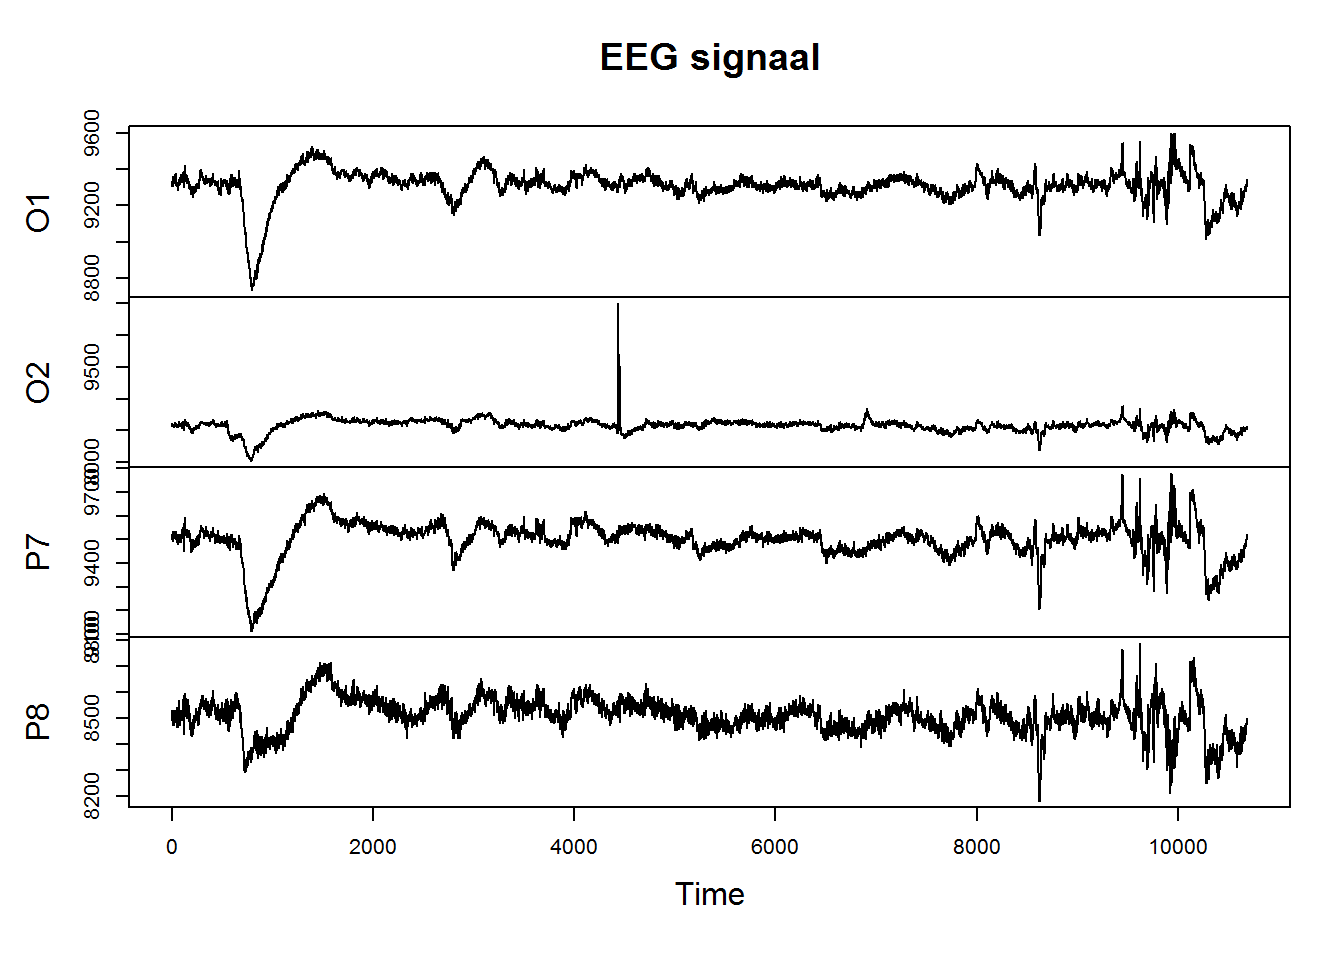
\includegraphics[width=10cm]{./eeg.png}
	\caption{Esialgne EEG signaal}
	\label{eeg}
\end{figure}



\chapter{Faktoranalüüs}

Kuna EEG signaalist eraldatud tunnuste puhul on tegemist aegreaga, siis vaatlused andmestikus ei ole sõltumatud. Seega tavalise faktoranalüüsi puhul ei saa me teha järeldusi väljaspoole antud andmestikku. Siin aga tuleb appi aegridade faktoranalüüs, mis ei tee vaatluste sõltumatuse eeldust, ning mida hiljem antud töös rakendatakse. Küll aga saame tavalist faktoranalüüsi kasutada antud andmestiku kokku surumiseks.

Lisaks prooviti töö käigus rakendada ka dünaamilist faktoranalüüsi, mis sobib samuti aegridade faktoranalüüsi tegemiseks, aga erinevalt aegridade faktoranalüüsist oli meetodi rakendamine ilma taustateadmisteta keerukas ning seetõttu dünaamilise faktoranalüüsiga tulemusteni antud töös ei jõutud.

Faktoranalüüsi prooviti rakendada ka EEG signaalile, aga nagu joonisel~\ref{eeg} näha, on erinevatest sensoritest saadud signaalid omavahel tugevalt korreleeritud ning seega saadakse tulemuseks üks faktor, mis on tugevalt seotud kõigi sensorite signaalidega. Seega EEG signaalile rakendatud faktoranalüüs (vähemasti antud sensorite korral) antud töös püstitatud küsimustele vastust leida ei aita.

Järgnevalt läheme EEG signaalist eraldatud tunnuste faktoranalüüsi juurde.

\section{Tunnuste ja faktorite arv}\label{faktorid}

Edasiseks analüüsiks valiti 6 tunnust (CCA\_f1, CCA\_f2, CCA\_f3 ning PSDA\_sum\_f1, PSDA\_sum\_f2, PSDA\_sum\_f2), iga käsu kohta kanoonilise korrelatsioonanalüüsi tulemus ja iga käsu kohta võimsusspekttri analüüsi üks tulemus. Kui kasutada mitut võimsusspektri analüüsi tunnust iga käsu kohta, siis kipub faktoranalüüs ära kirjeldama just võimsusspektri analüüsi meetodid ning seejuures jätab kanoonilise korrelatsioonanalüüsi meetodi praktiliselt kirjeldamata. Seda me aga ei taha, kuna kanoonilise korrelatsioonanalüüsi meetod on käsu kindlaks tegemisel täpsem kui võimsusspektri analüüs.

Interpreteerimise huvides valiti faktorite arvuks kolm, kuna andmed on juhu kohta, kus kasutaja sai edastada kolme erinevat käsku. Sel juhul iga saadud faktor võiks vastata ühele käsule ning saame proovida kasutada kasutaja edastatud käsu kindlaks tegemiseks hoopis faktorite väärtuseid, mitte tunnuste omi. Vähemate või rohkemate tunnuste korral on interpreteerimine problemaatiline ning tõenäoliselt ei saa ka sel juhul faktorskoore käsu kindlaks tegemisel kasutada.

Nelja faktori korral tekkis üks faktor, mis on tugevalt seotud ainult kanoonilise korrelatsioonanalüüsi meetodiga. Selline faktor ei aita andmestikku kokku suruda, kuna otsime pigem meetodite vahelisi seoseid. Seega valimegi kolm faktorit.

Teine idee tunnuste ja faktorite arvu valimiseks oli, et valime tunnused, mis iseloomustavad ainult ühte käsku ehk näiteks käsu 1 puhul valime alamhulga tunnustest CCA\_f1, PSFA\_sum\_f1, PSFA\_h1\_f1, PSFA\_h2\_f1 ning teeme faktoranalüüsi ühe faktori korral. Sellisel juhul on faktoranalüüs sunnitud just ühe käsu tunnused omavahel kombineerima ning ei saa tekkida mitte-interpreteeritavust erinevate käskude tunnuste kombineerimise tõttu. Antud idee ei mahtunud kahjuks antud töö skoopi.

\begin{figure}[h!]
	\centering
	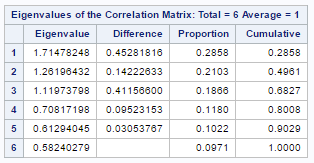
\includegraphics{eigen.png}
	\caption{Korrelatsioonimaatriksi omaväärtused. Näiteks omaväärtused \textgreater 1 tingimuse järgi saaksime ka siit 3 faktorit.}
\end{figure}

\section{Faktorlahend}

Faktorlahendi leidmiseks võrreldi nelja meetodit: peakomponentide meetod, peafaktorite meetod, iteratiivne peafaktorite meetod ning aegridade faktoranalüüs, mis põhines suurima tõepära meetodil. Leitud faktorkaalud ning kommunaliteedid on visualiseeritud joonisel~\ref{kaalud} ning tabelina toodud lisas. Jooniselt näeme, et peafaktorite meetodid annavad väga sarnaseid tulemusi. Ka peakomponentide meetod väga palju peafaktorite meetodist ei erine, kuid nagu oodatud, kirjeldab ära suurema tunnuste dispersioonist ning seega omapärad on väiksemad. Suurima tõepära meetod head tulemust ei andnud, iga faktor on seotud peamiselt ainult ühe tunnusega ja seega tunnuseid kokku ei suruta.

Teised headuse näitajad on toodud joonisel~\ref{head}. Nagu näeme, on peafaktorite meetodi summaarne kirjeldatus hea ning ka teised näitajad on piisavalt väikesed. Peafaktorite meetod, nagu oodatud, on aga saavutanud väga väikesed jääkkorrelatsiooni ja osakorrelatsiooni maatriksi diagonaaliväliste elementide summad. 

Kuna aga peafaktorite meetod kirjeldab suhteliselt halvasti tunnust CCA\_f3 ja ka teiste tunnuste kommunaliteedid on üpris väikesed, siis valime lahendiks peakomponentide meetodi tulemuse.

\begin{figure}[h!]
	\centering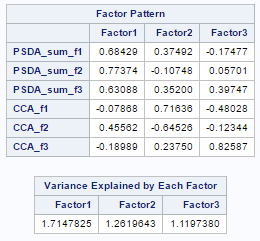
\includegraphics{kaalud.png}
	\caption{Peakomponentide meetodil saadud faktorkaalud.}
\end{figure}

\begin{figure}[h!]
	\centering
	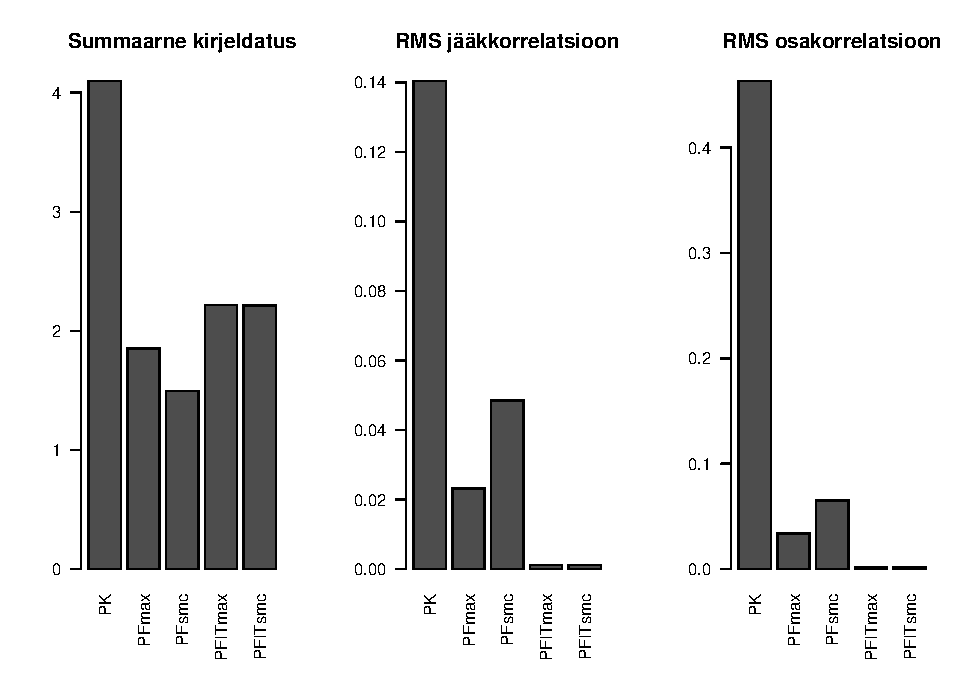
\includegraphics[height=10cm]{kaalud3.pdf}
	\caption{Erinevate meetodite summaarne kirjeldatus, RMS jääkkorrelatsiooni maatriksi diagonaalivälistest elementidest, RMS osakorrelatsiooni maatriksi diagonaalivälistest elementidest.}\label{head}
\end{figure}

\section{Pööramine}

Et saavutada faktorstruktuur, mis vastab peatükis~\ref{faktorid} seatud tingimusele, et iga faktor vastab ühele käsule, kasutame Prokrustese pööramist. Varimax ning teised tuntud meetodid ei andnud piisavalt hästi interpreteeritavat tulemust. Faktorite ning tunnuste korrelatsioonid on toodud joonisel~\ref{prokrustes}. Näeme, et soovitud struktuur on päris hästi saavutatud. Esimesel faktoril on suured korrelatsioonid tunnustega PSDA\_sum\_f1 ja CCA\_f1, teisel faktoril on suured korrelatsioonid tunnustega PSDA\_sum\_f2 ja CCA\_f2 ning kolmandal tunnustega PSDA\_sum\_f3 ja CCA\_f3.

\begin{figure}[h!]
	\centering
	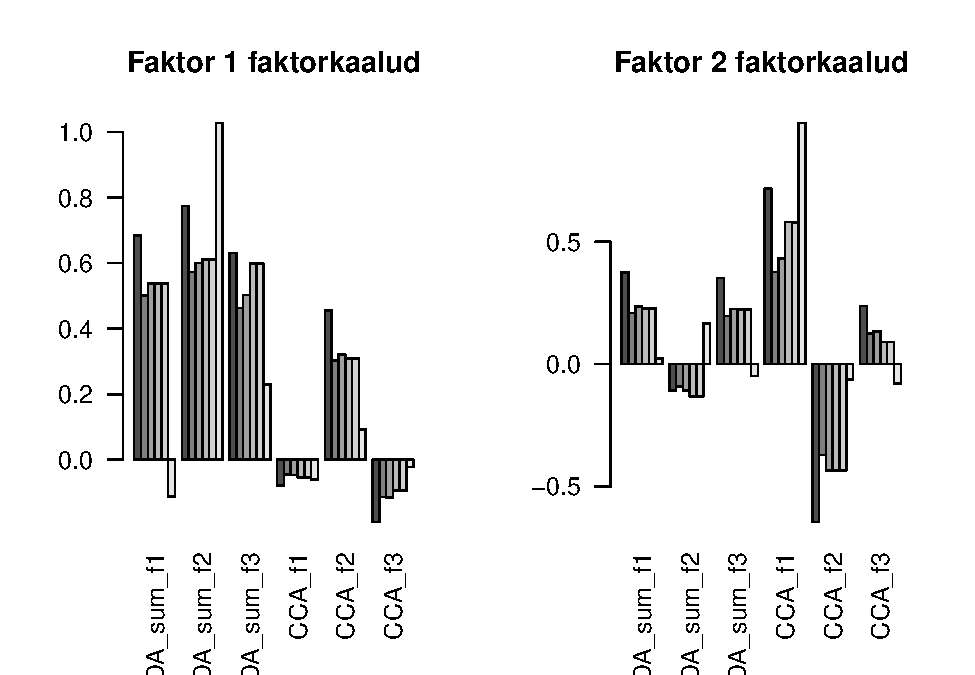
\includegraphics[height=10cm]{kaalud1.pdf}
	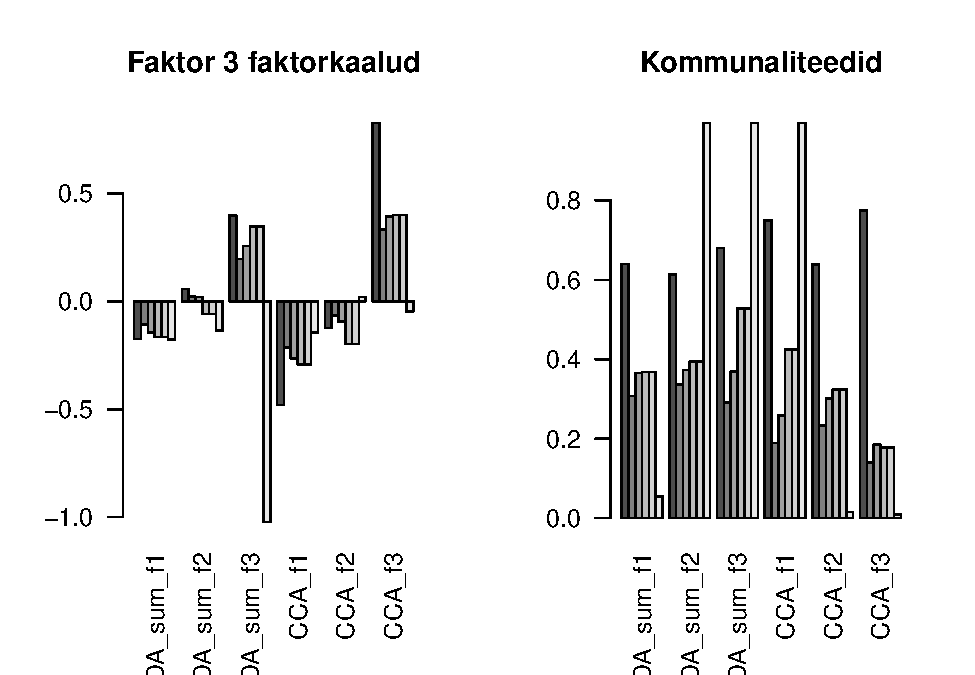
\includegraphics[height=10cm]{kaalud2.pdf}
	\caption{Faktorkaalud ja kommunaliteedid. Meetodid on kodeeritud toonidena tumedamalt toonilt heledamale (vasakult paremale) järgnevalt: peakomponendid, peafaktorid max, peafaktorid smc, iteratiivne peafaktor max, iteratiivne peafaktor smc, aegridade faktoranalüüs suurima tõepära meetodil.}\label{kaalud}
\end{figure}

\begin{figure}[h!]
	\centering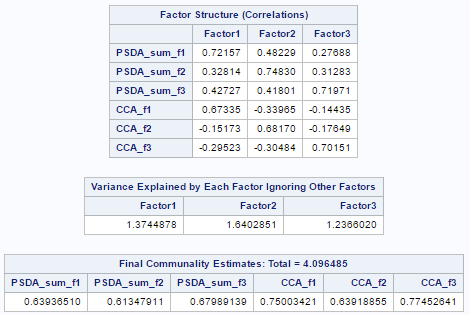
\includegraphics{prokrustes.png}
	\caption{Prokrustese pööramise tulemusel saadud faktorstruktuur.}\label{prokrustes}
\end{figure}

Arvutame ka faktorite skoorid. Seda saame teha korrutades tunnuste vektori faktorskooride maatriksiga, aga SAS arvutab need ka automaatselt. Tulemus on toodud joonisel~\ref{skoorid}. Kuna aga antud jooniselt on raske midagi välja lugeda, siis järgnevalt proovime saadud faktorskooride põhjal ka kasutaja edastatud käsku kindlaks teha, et näha, kas antud tunnuste kokku surumisest oli ka kasu.

\begin{figure}[h!]
	\centering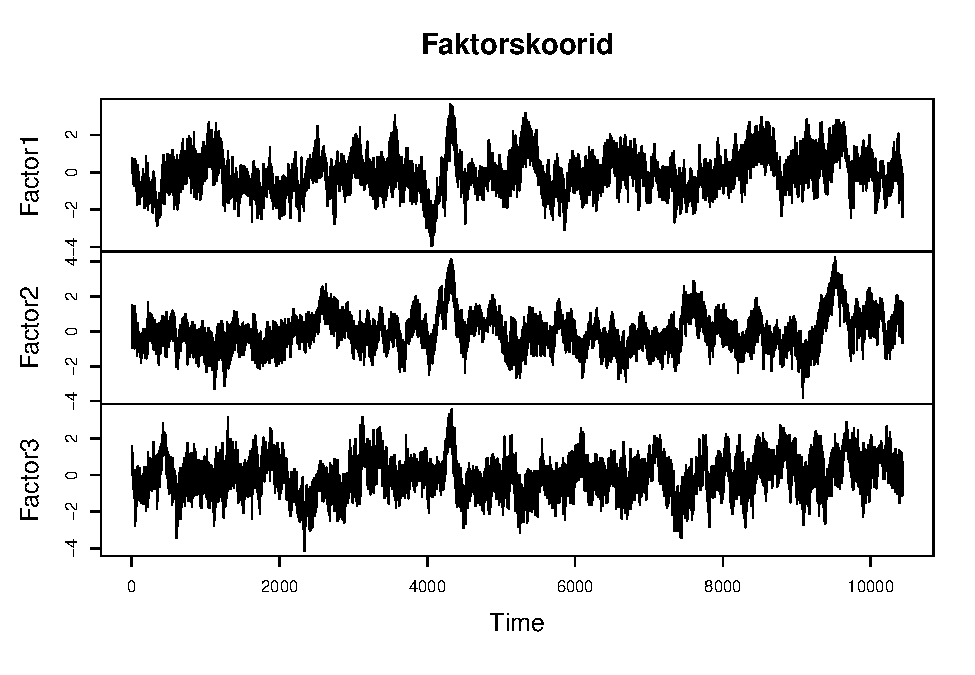
\includegraphics[height=10cm]{skoorid.pdf}
	\caption{Faktorskoorid.}\label{skoorid}
\end{figure}

\section{Faktorskooride põhjal klassifitseerimine}

Järgnevalt proovime arvutatud faktorskooride põhjal kasutaja edastatud käsku kindlaks teha. Selleks kasutame kõige lihtsamat klassifitseerijat, mis teeb valiku lävendi põhjal. Kui faktorskoor on suurem kui lävend, siis ennustame, et kasutaja proovis faktorile vastavat käsku edastada. Kui lävend on väiksem, siis kasutaja ei proovinud antud käsku edastada. Antud meetod on väga ebatäpne, kuid siiski saame seda võrrelda esialgsete tunnuste põhjal klassifitseerimisega. 

Binaarse klassifitseerija headust saab visualiseerida ROC kõveraga, millelt on näha kuidas sõltuvad klassifitseerija tundlikkus ja spetsiifilisus üksteisest. Mida kõrgemalt ROC kõver läheb, seda parem on klassifitseerija. Joonisel~\ref{roc} näeme, et antud väga naiivne klassifitseerija eriti häid tulemusi ei anna. Kõige paremini töötab klassifitseerimine kanoonilise korrelatsioonanalüüsi tunnuste puhul. 

\begin{figure}[h!]
	\centering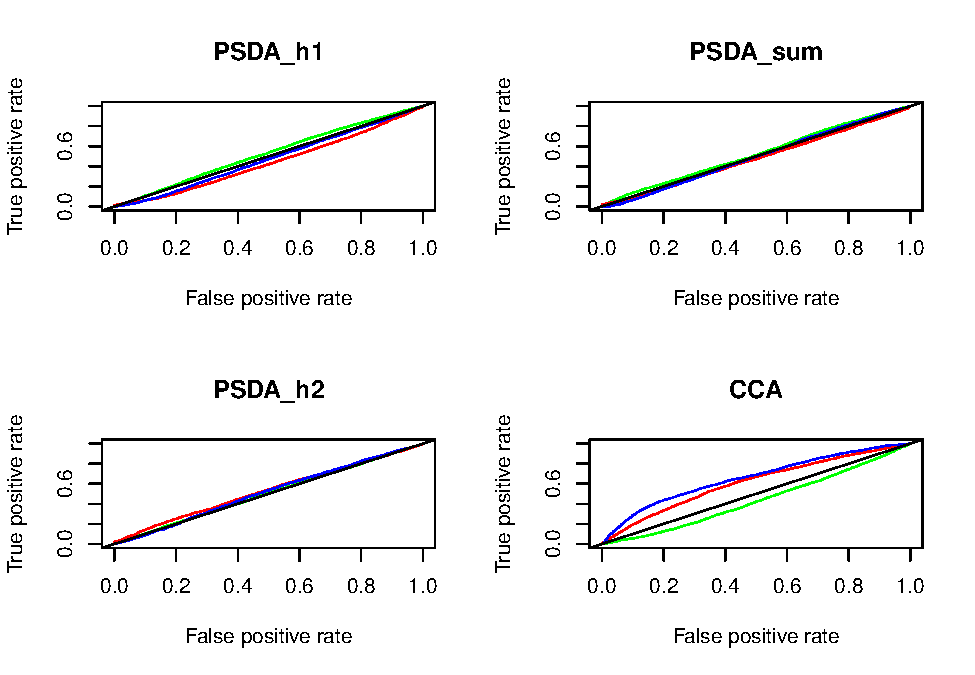
\includegraphics{roc.pdf}
	\caption{Esialgsete tunnuste põhjal klassifitseerimine. Roheline joon vastab käsule 1 (6.67 Hz), punane joon käsule 2 (7.5 Hz) ja sinine joon käsule 3 (8.57 Hz).}\label{roc}
\end{figure}

\begin{figure}[h!]
	\centering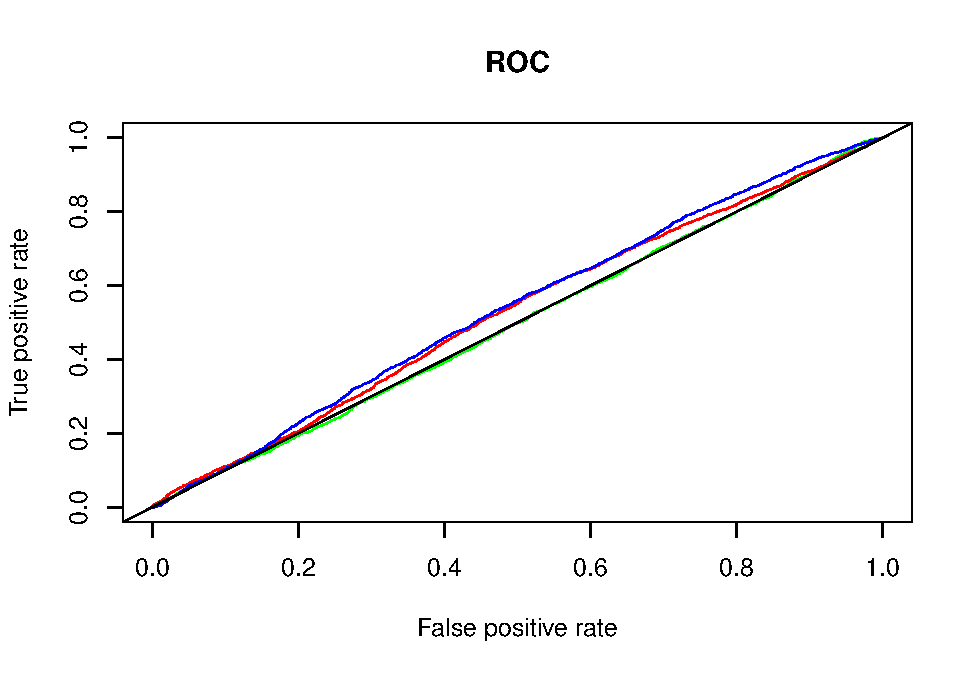
\includegraphics[width=12cm]{rocfac.pdf}
	\caption{Faktorskooride põhjal klassifitseerimine.}\label{rocfac}
\end{figure}

Joonisel~\ref{rocfac} on aga kujutatud faktorskooride põhjal klassifitseerimine. Näeme, et tulemus on parem kui ainult võimsusspektri meetodiga eraldatud tunnuste põhjal klassifitseerimine. Seega on lootust, et faktoranalüüsiga leitud faktorskooride põhjal klassifitseerimine töötab ka keerulisemate ja täpsemate klassifitseerijate korral.

\chapter{Kokkuvõte}

Antud töös kasutati faktoranalüüsi et suruda kokku EEG signaalist eraldatud tunnused, mille põhjal AAL proovib otsustada, millist käsku kasutaja arvutile edastada soovib. Tunnuste kokku surumine muudaks lihtsamaks käsu kindlaks tegemise, kuna vähemate tunnuste korral tuleb vähem manuaalselt otsida ja muuta parameetreid. Kui faktorlahendiks on nii paljude faktoritega struktuur kui palju on edastatavaid käske ning iga faktor on tugevalt seotud ühe käsuga (st vastava käsu jaoks eraldatud tunnustega), siis on võimalik faktorlahendit interpreteerida ning tõenäoliselt on võimalik ka faktorskoore kasutada klassifitseerimiseks.

Projekti edasi arendamise esimene samm oleks teha parem klassifitseerimise meetod ning vaadata, kuidas faktorskooride põhjal klassifitseerimine parema meetodi puhul töötab. Teiseks tuleks proovida peatükis~\ref{faktorid} mainitud ideed kasutada ainult ühte faktorit ning ühe käsuga seotud tunnuseid.

Sain antud projekti käigus ideid oma AALi edasi arendamiseks ning loodetavasti viib mõni neist ka hea tulemuseni.

\appendix
\chapter{Lisa}\label{lisa1}

Andmed ning kõik projekti jaoks kasutatud koodid on kättesaadavad projekti koodirepositooriumist\footnote{https://github.com/kahvel/MAProject}. Järgnevalt on aga toodud näited andmestikust ning kasutatud olulisemad koodi osad

\begin{verbatim}
data data; /* Andmete sisse lugemine */
infile 'test5_results_2_all.csv';
input ID PSDA_sum_f1 PSDA_sum_f2 PSDA_sum_f3
         PSDA_h1_f1 PSDA_h1_f2 PSDA_h1_f3
         PSDA_h2_f1 PSDA_h2_f2 PSDA_h2_f3
         CCA_f1 CCA_f2 CCA_f3;
run;

data TARGET; /* Pööramise soovitud tulemus */
Input _NAME_ $ PSDA_sum_f1 PSDA_sum_f2 PSDA_sum_f3
               CCA_f1 CCA_f2 CCA_f3;
list;cards;
FACTOR1 1 0 0 1 0 0
FACTOR2 0 1 0 0 1 0
FACTOR3 0 0 1 0 0 1
;
run;
/* Peakomponentide meetod pööramisega */
proc factor data=data method=prin priors=one rotate=procrustes
            target=target residuals nfactors=3;
var PSDA_sum_f1 PSDA_sum_f2 PSDA_sum_f3 CCA_f1 CCA_f2 CCA_f3;
run;
/* Peafaktorite meetod max */
proc factor data=data method=prin priors=max residuals nfactors=3;
var PSDA_sum_f1 PSDA_sum_f2 PSDA_sum_f3 CCA_f1 CCA_f2 CCA_f3;
run;
/* Peafaktorite meetod smc */
proc factor data=data method=prin priors=smc residuals nfactors=3;
var PSDA_sum_f1 PSDA_sum_f2 PSDA_sum_f3 CCA_f1 CCA_f2 CCA_f3;
run;
/* Iteratiivne peafaktorite meetod max */
proc factor data=data method=prinit priors=max residuals nfactors=3 maxiter=1000;
var PSDA_sum_f1 PSDA_sum_f2 PSDA_sum_f3 CCA_f1 CCA_f2 CCA_f3;
run;
/* Iteratiivne peafaktorite meetod smc */
proc factor data=data method=prinit priors=smc residuals nfactors=3 maxiter=1000;
var PSDA_sum_f1 PSDA_sum_f2 PSDA_sum_f3 CCA_f1 CCA_f2 CCA_f3;
run;
\end{verbatim}
Näide EEG signaali andmestiku kohta
\begin{longtable}[c]{@{}rrrr@{}}
	\toprule
	O1 & O2 & P7 & P8\tabularnewline
	\midrule
	\endhead
	9317 & 8587 & 9507 & 8518\tabularnewline
	9327 & 8604 & 9510 & 8526\tabularnewline
	9334 & 8613 & 9517 & 8519\tabularnewline
	9334 & 8611 & 9521 & 8531\tabularnewline
	9326 & 8598 & 9512 & 8529\tabularnewline
	9311 & 8580 & 9507 & 8506\tabularnewline
	\bottomrule
\end{longtable}
Kasutatud käskude sagedused
\begin{longtable}[c]{@{}rr@{}}
	\toprule
	ID & Frequency\tabularnewline
	\midrule
	\endhead
	1 & 6.666667\tabularnewline
	2 & 7.500000\tabularnewline
	3 & 8.571429\tabularnewline
	\bottomrule
\end{longtable}
Näide EEG signaalist eraldatud tunnuste kohta
\begin{longtable}[c]{@{}rrrrrr@{}}
	\toprule
	PSDA\_sum\_f1 & PSDA\_sum\_f2 & PSDA\_sum\_f3 & CCA\_f1 & CCA\_f2 &
	CCA\_f3\tabularnewline
	\midrule
	\endhead
	3.896971 & 4.119254 & 4.575920 & 0.3028430 & 0.2741514 &
	0.2669149\tabularnewline
	4.474294 & 4.549097 & 4.406292 & 0.3335525 & 0.2597220 &
	0.2564238\tabularnewline
	5.010334 & 4.474692 & 4.151357 & 0.3411201 & 0.2703358 &
	0.2189455\tabularnewline
	4.915839 & 4.368423 & 4.323578 & 0.3289583 & 0.3110394 &
	0.2421184\tabularnewline
	4.867986 & 4.590158 & 4.520489 & 0.3165068 & 0.3610076 &
	0.2756416\tabularnewline
	4.702446 & 4.580038 & 4.602424 & 0.3026591 & 0.3378599 &
	0.2960716\tabularnewline
	\bottomrule
\end{longtable}
Näide juhuslikult genereeritud käskude järjendi kohta ehk millal kasutaja mingit käsku edastas
\begin{longtable}[c]{@{}rrr@{}}
	\toprule
	Start & Stop & Target\tabularnewline
	\midrule
	\endhead
	1 & 512 & 2\tabularnewline
	513 & 576 & 1\tabularnewline
	577 & 1312 & 3\tabularnewline
	1313 & 2048 & 1\tabularnewline
	2049 & 2688 & 2\tabularnewline
	2689 & 3392 & 1\tabularnewline
	3393 & 5088 & 2\tabularnewline
	5089 & 5568 & 3\tabularnewline
	\bottomrule
\end{longtable}
\newpage
Andmete failid (koodirepositooriumis)
\begin{itemize}
	\item \texttt{test5\_2.csv} - EEG signaal;
	\item \texttt{test5\_freq\_2.csv} - kasutatud käskude sagedused;
	\item \texttt{test5\_targets\_2.csv} - millal kasutaja mingit käsku edastas;
	\item \texttt{test5\_results\_2\_all.csv} EEG signaalist eraldatud tunnused.
\end{itemize}
Aegridade faktoranalüüsi Ris
\begin{verbatim}
library(tsfa)
result_data <- read.csv("test5_results_2_all.csv", header=TRUE, sep=" ")
fit = estTSFmodel(ts(result_data), 3) # 3=faktorite arv
summary(fit)
\end{verbatim}
Dünaamiline faktoranalüüs Ris 6 tunnuse ja 3 faktoriga
\begin{verbatim}
library(MARSS)
result_data <- read.csv("test5_results_2_all.csv", header=TRUE, sep=" ")
Z.vals = list(
"z11", 0, 0,
"z21", "z22", 0,
"z31", "z32", "z33",
"z41", "z42", "z43",
"z51", "z52", "z53",
"z61", "z62", "z63"
)
N.ts = 6
Z = matrix(Z.vals, nrow=N.ts, ncol=3, byrow=TRUE)
Q = B = diag(1,3)
R.vals = list(
"r11",0,0,0,0,0,
0,"r22",0,0,0,0,
0,0,"r33",0,0,0,
0,0,0,"r44",0,0,
0,0,0,0,"r55",0,
0,0,0,0,0,"r66")
R = matrix(R.vals, nrow=N.ts, ncol=N.ts, byrow=TRUE)
x0 = U = matrix(0, nrow=3, ncol=1)
A = matrix(0, nrow=6, ncol=1)
V0 = diag(5,3)
dfa.model = list(Z=Z, A="zero", R=R, B=B, U=U, Q=Q, x0=x0, V0=V0)
cntl.list = list(maxit=50)
tulemus = MARSS(t(as.matrix(result_data)), model=dfa.model, control=cntl.list)
\end{verbatim}


\end{document}
